\section{Measured Results}\label{sec:results}
The realised circuit in \cref{sec:implementation} was designed with a PGA and the mesaured results are for the combined CCIA and PGA. The IRN of the AFE (with and without chopping) was measured with an audio analyser (\textit{SR1 — Dual-domain audio analyser from Stanford Research Systems}) while the AFE's inputs were grounded and the gain was set to maximum ( 55.6 dB). \cref{fig:CCIA_IRN} shows the simulated and measured IRN with and without chopping. At \SI{1}{\kilo\hertz}, the AFE's IRN was \SI{2.07}{\nano\volt\per\sqrt{\hertz}} with a chopping frequency at \SI{1.28}{\mega\hertz}. The simulated result is a pnoise simulation. The AFE achieved a maximum DC gain of \SI{55.6}{\deci\bel} within a bandwidth of \SI{100}{\hertz} - \SI{60}{\kilo\hertz}, featuring a high-pass (HP) filter pole at \SI{2}{\hertz} as shown in \cref{fig:CCIA_GAIN}. 
% \begin{figure} [!htbp]
%     \centering
%     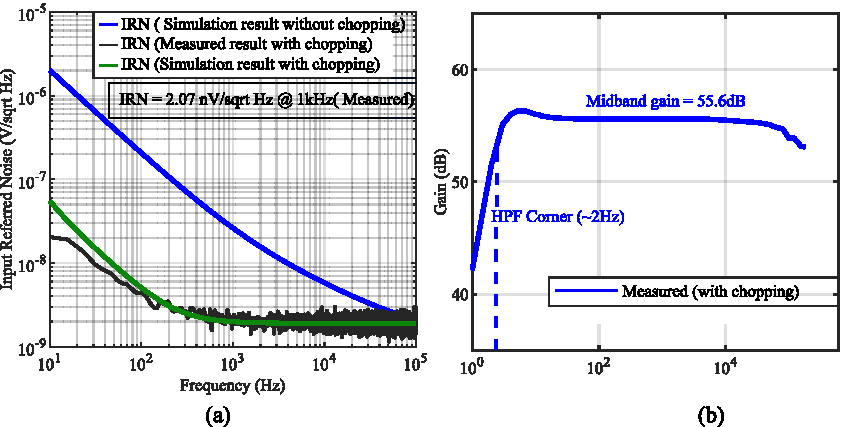
\includegraphics[ width = \columnwidth]{img/Chip_measurement_AFE_NEW_SCH_1.pdf} 
%     \caption{(a) Simulated and measured AFE input-referred noise density with and without chopping. (b) Measured DC gain of AFE.\cite{srivastava20243d}}
%     \label{chip_char_IRN}
% \end{figure}
\begin{figure}[!htbp]
        \centering
        \begin{subfigure}[c]{0.49\linewidth}
            \centering
            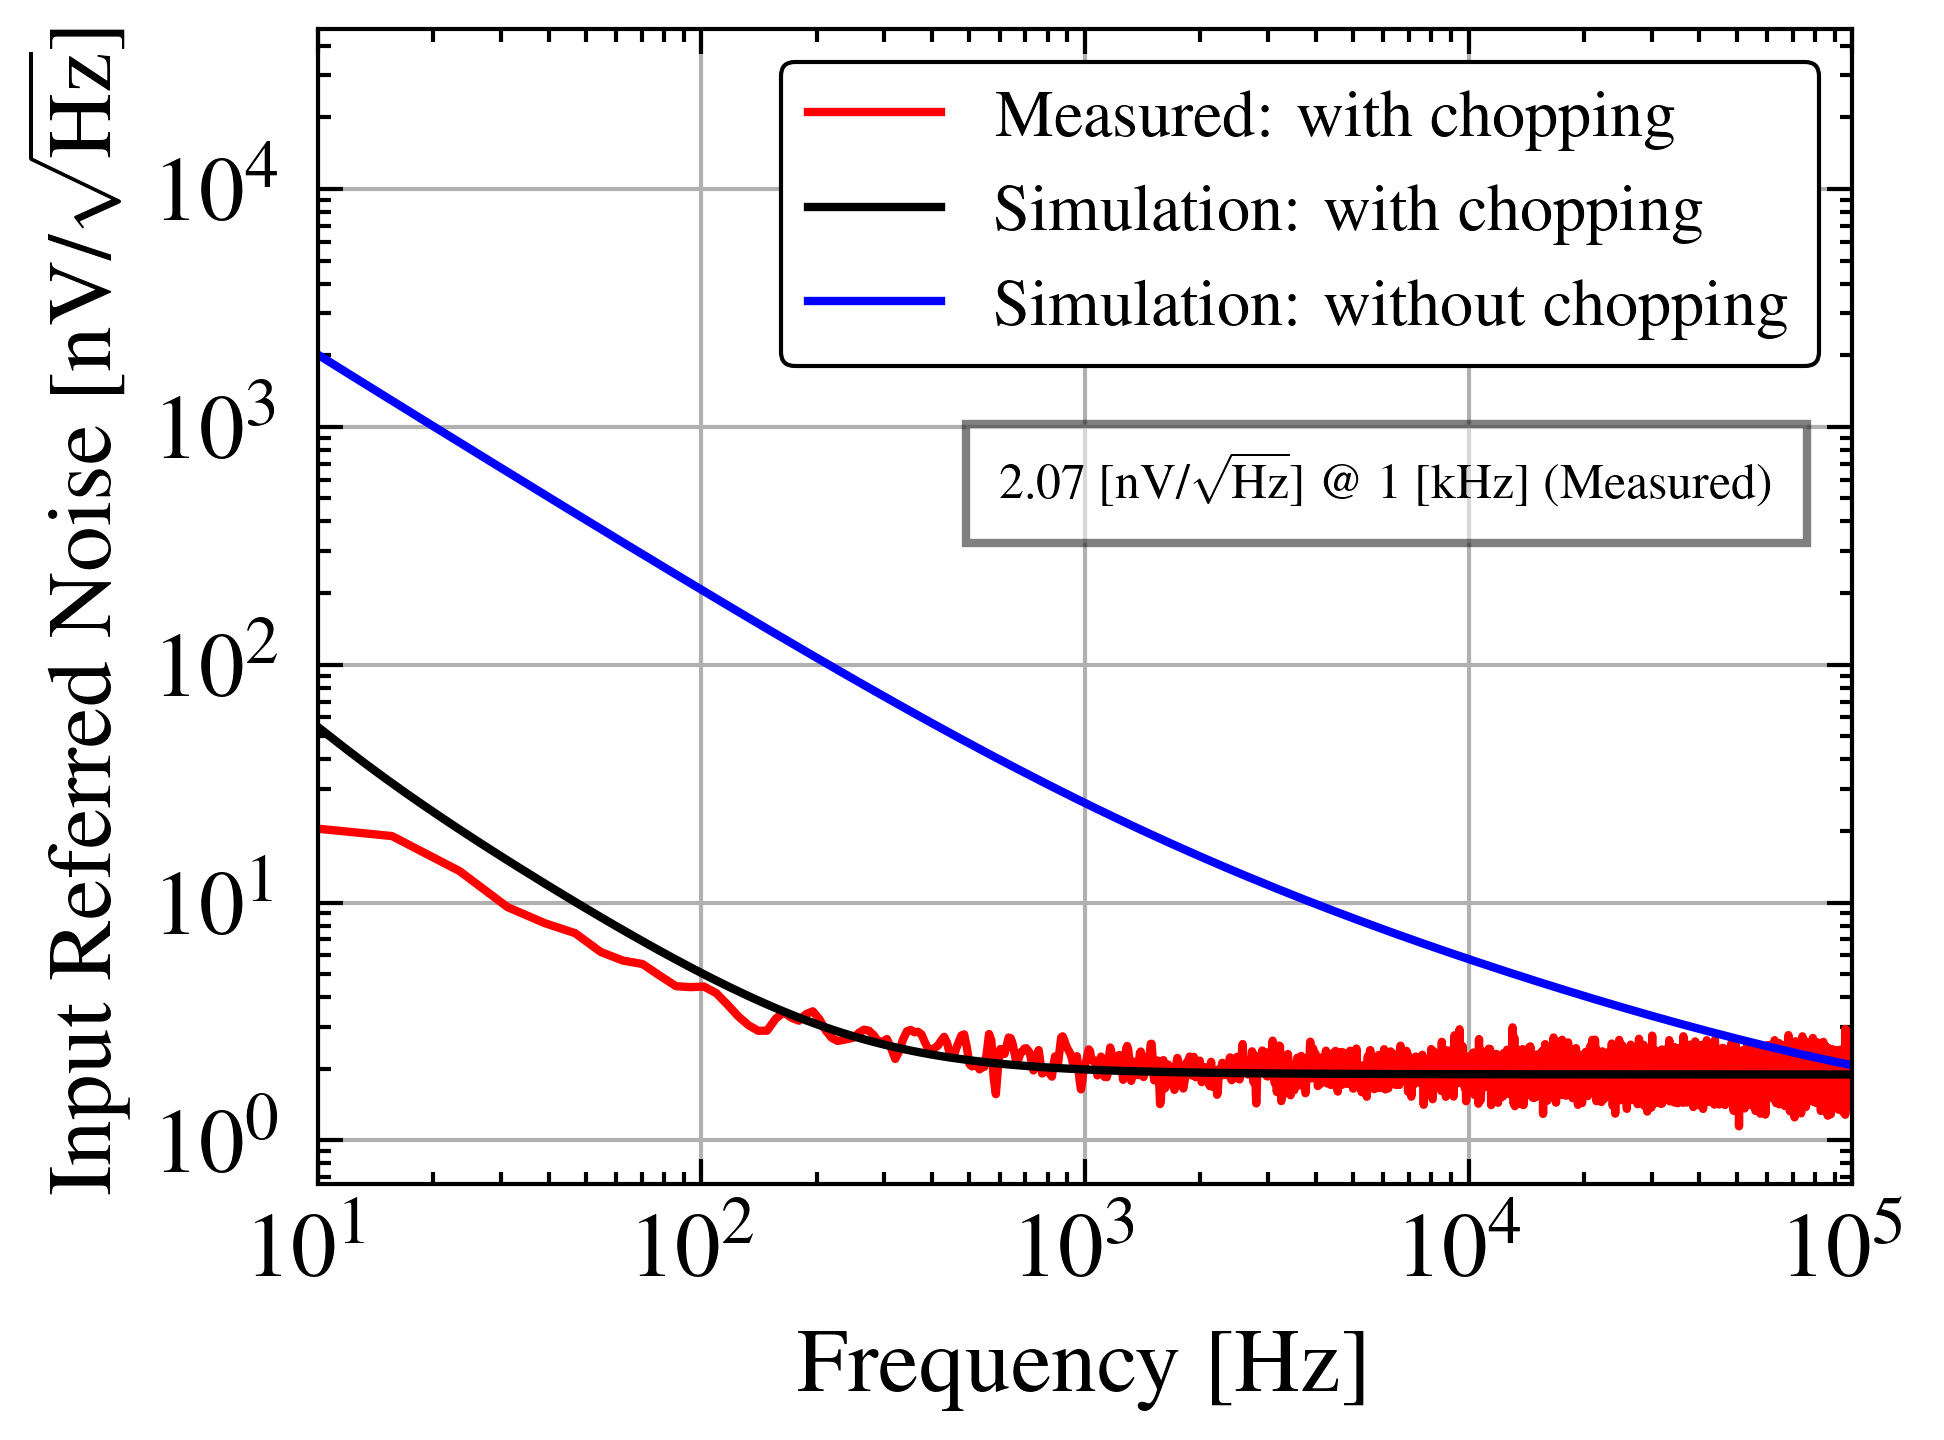
\includegraphics[width=\linewidth]{img/IRN_MEASURED.png}
            \caption[]%
            {{\small }}
            \label{fig:CCIA_IRN}
        \end{subfigure}
        \hfill
        \begin{subfigure}[c]{0.49\linewidth}  
            \centering 
            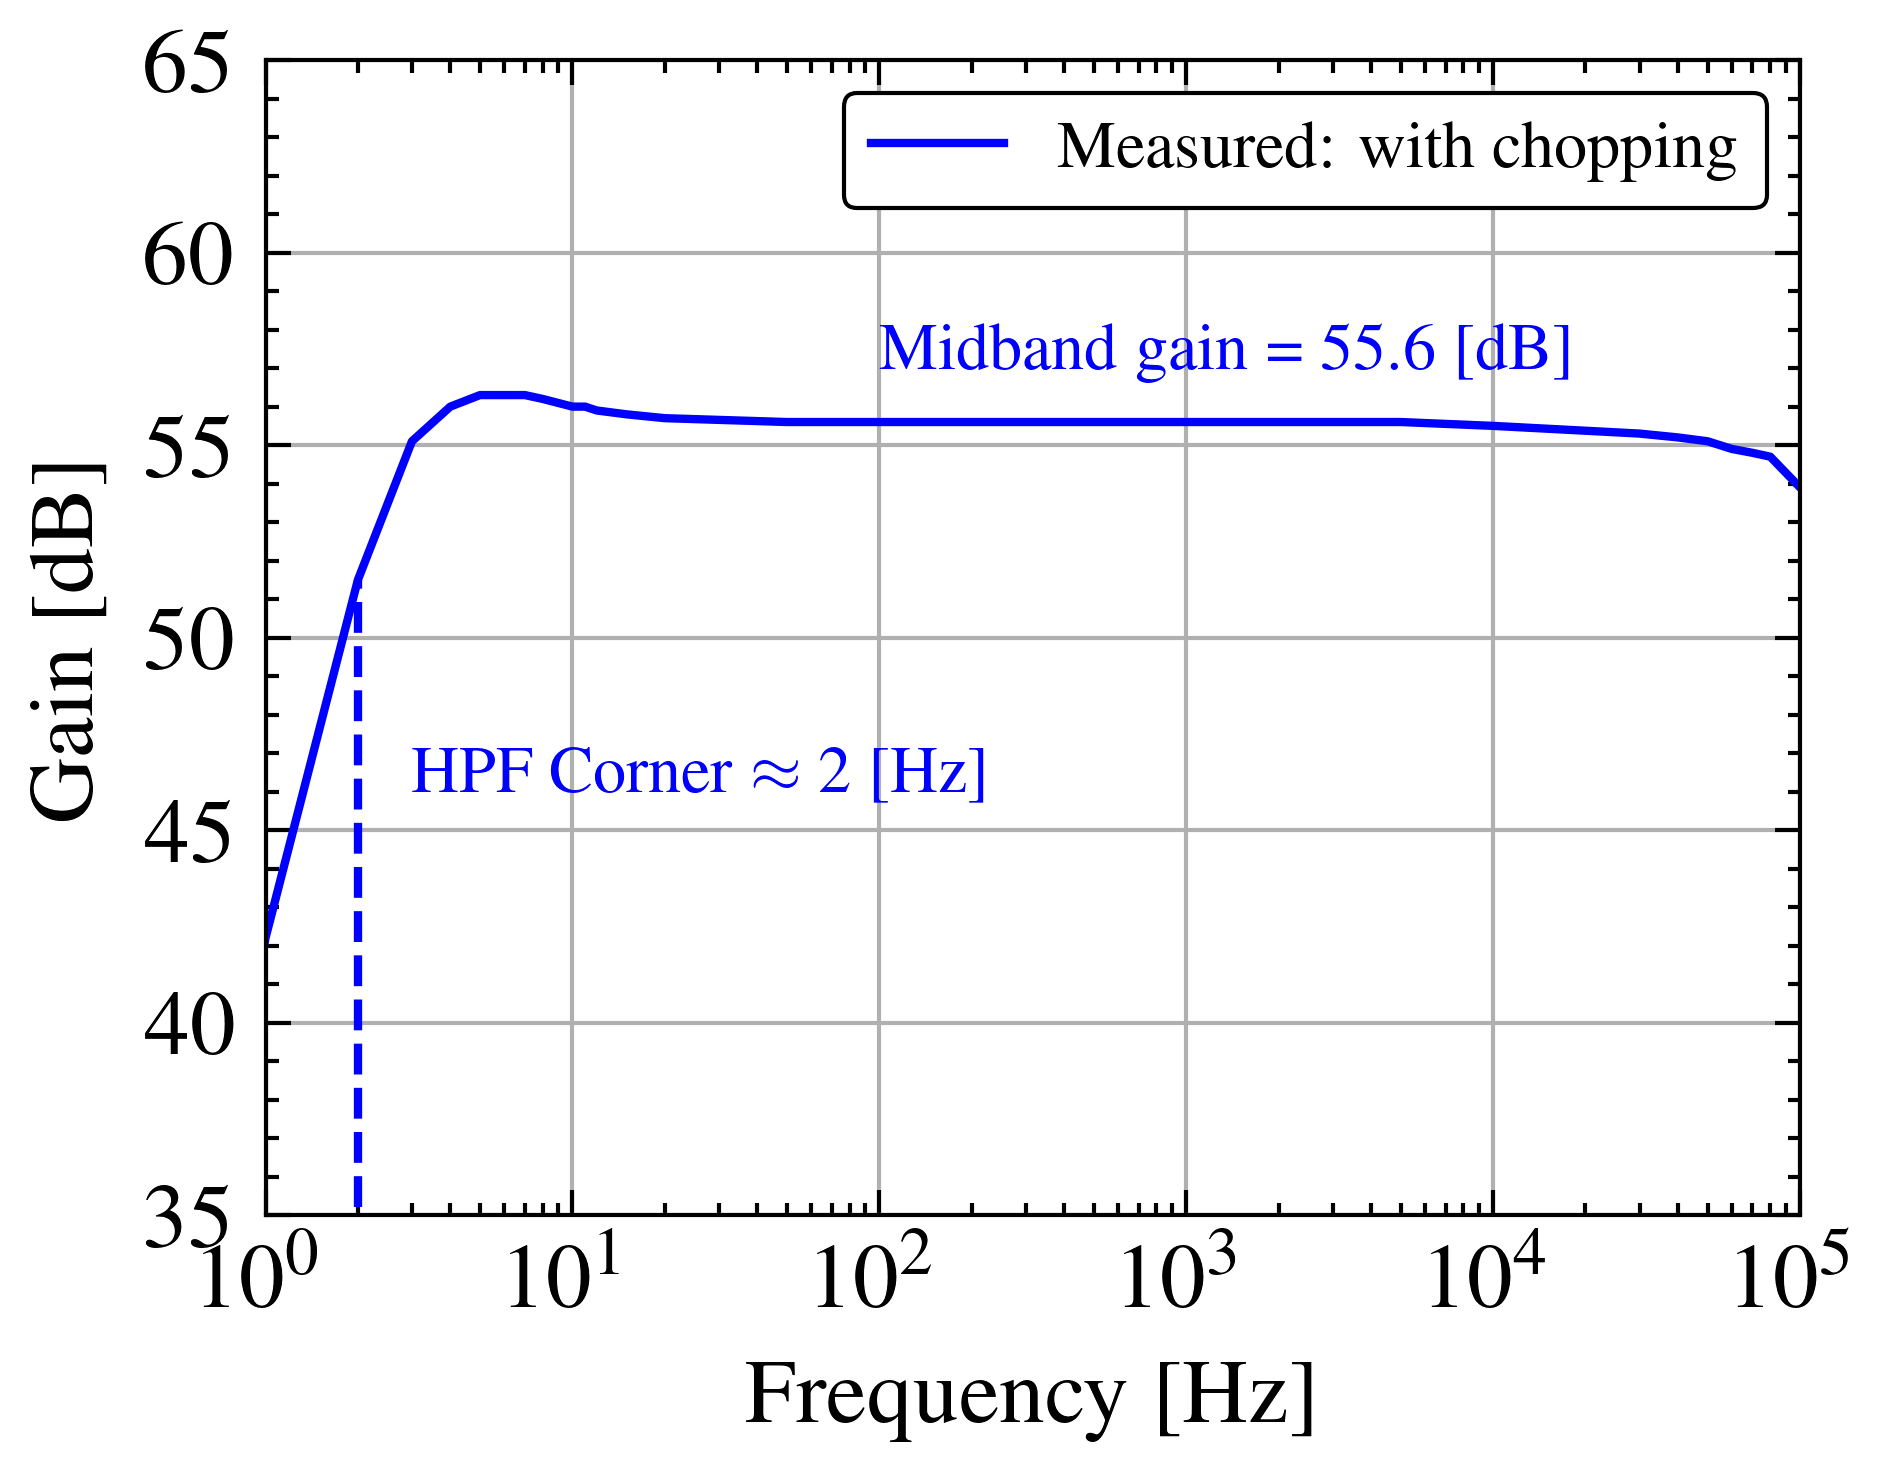
\includegraphics[width=\linewidth]{img/GAIN_MEASURED.png}
            \caption[]%
            {{\small }}
            \label{fig:CCIA_GAIN}
        \end{subfigure}
        \caption[ Don't write caption here ]
        {(a) Simulated and measured AFE input-referred noise density with and without chopping. \cite{srivastava20243d} (b) Measured DC gain of AFE. } 
        \label{fig:chip_char_IRN}
\end{figure}
%It is worth noting that the simulation result was obtained without chopping. As the open-loop amplifier gain at the chopping frequency is less than the response at close to DC the measured result should be close to the simulated result at the chopping frequency of 500 kHz, as shown in Fig.~\ref{chip_char_IRN}(b).
The peaking in the gain response is caused by the AC coupling at the input as shown in \Cref{fig:DL-CCIA} and the inter-stage AC coupling. The composite bi-quad pole-zero responses create the peaking. The AFE consumes \SI{2.6}{\milli\ampere} and occupies \SI{0.18}{\milli\metre^2} active area. A comparison with the state-of-the-art for CCIA is presented in Table~\ref{SOFA_AFE}.

\begin{table}[!htb]
\begin{adjustbox}{width=\linewidth,center}
\begin{threeparttable}
\centering
\caption{Comparison with the state-of-the-art}
\label{SOFA_AFE}
%\resizebox{\columnwidth}{!}{%
%\renewcommand{\footnotesize}{\tiny}
\begin{tabular}{|c|c|c|c|c|}
%\begin{tabular}{|*{8}{c|}}
\hline
Metrics    & This work & \cite{Jiang-8588386}  &  \cite{Maruyama-7516659}  &  \cite{Shen-8008461}   \\ \hline
CMOS technology {[}nm{]}       & 65   & 180    & 180 & 180     \\ \hline
Architecture & CCIA & CCIA+CTDSM & 3-Opamp & Inverter-stacking \\ \hline
Active Area  {[}$mm^2${]}    & 0.18\tnote{a} & 0.73  & 0.22  & 0.02      \\ \hline
Supply Voltage {[}V{]} & 1.2 & 1.8 & 1.55 & 1      \\ \hline
Current {[}mA{]} & 1.48\tnote{b}  & 1.2    & 1.3      & 0.00025   \\ \hline
Input Noise Density {[}$nV/\sqrt{Hz}${]}  & 2.07 & 3.7  & 8.2  & 55       \\ \hline
Input Offset {[}$\mu V${]}   & 1.25  & 7 & N.R. & N.R. \\ \hline
CMRR  {[}dB{]}     & 82 & 134   & N.R.  & 82 \\ \hline
NEF/PEF\tnote{c} & 3.12/11.68  & 5/44      & 11.4/201  & 1.07/1.14    \\ \hline
\end{tabular}
%}
% \par\medskip
    \footnoterule
    \begin{tablenotes}
    {\fontsize{6pt}{7pt}\selectfont
     \item [a] CCIA and PGA area included 
      \item [b] CCIA current only
    \item [c] PEF = VDD*$NEF^2$ 
    \item N.R.: Not reported}
\end{tablenotes}
\end{threeparttable}
\end{adjustbox}
\end{table}

%\begin{figure} [!htbp]
%    \centering
%    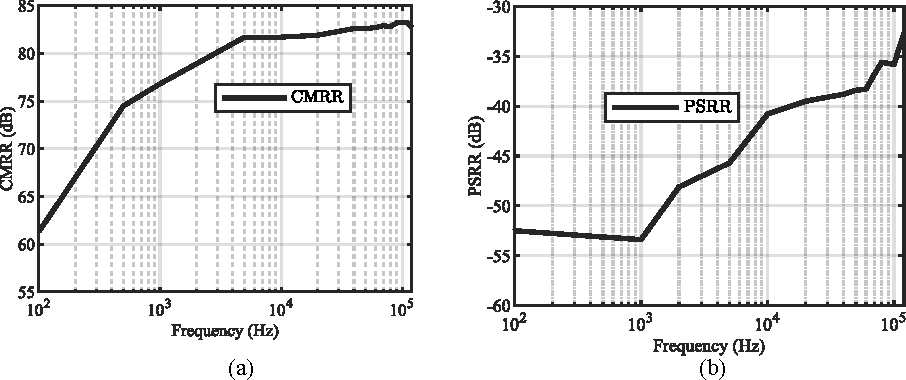
\includegraphics[ width = \columnwidth]{img/Chip_measurement_AFE_NEW_CMRR_PSRR.pdf} 
%    \caption{(a) Measured CMRR of AFE. (d) Measured PSRR of AFE without LDO}
%    \label{chip_char_CMRR}
%\end{figure}